\begin{appendix} %Anhang
    \section{Bilddokumentation des Angriffs}

    Dieser Anhang dokumentiert den Angriff zusätzlich anhand manueller Screenshots.
    Die Abbildungen dienen nicht als eigenständiger Nachweis der Schwachstelle,
    sondern als visuelle Ergänzung zur in Kapitel \ref{sec:analyse} beschriebenen
    PoC-Analyse und zu den automatisierten Tests aus Kapitel \ref{sec:testing}.

    \subsection{UI-basierte Reproduktion}

    Die UI-Screenshots zeigen den Angriff in einer realistischen Benutzerperspektive:
    Zunächst wird durch das Opfer ein Fahrzeug angelegt, danach wird dieses Objekt
    durch einen Benutzer einer fremden Organisation ausserhalb seines erlaubten
    Mandantenkontexts sichtbar gemacht beziehungsweise trotz Löschung weiterhin
    angezeigt.

    \begin{figure}[H]
        \centering
        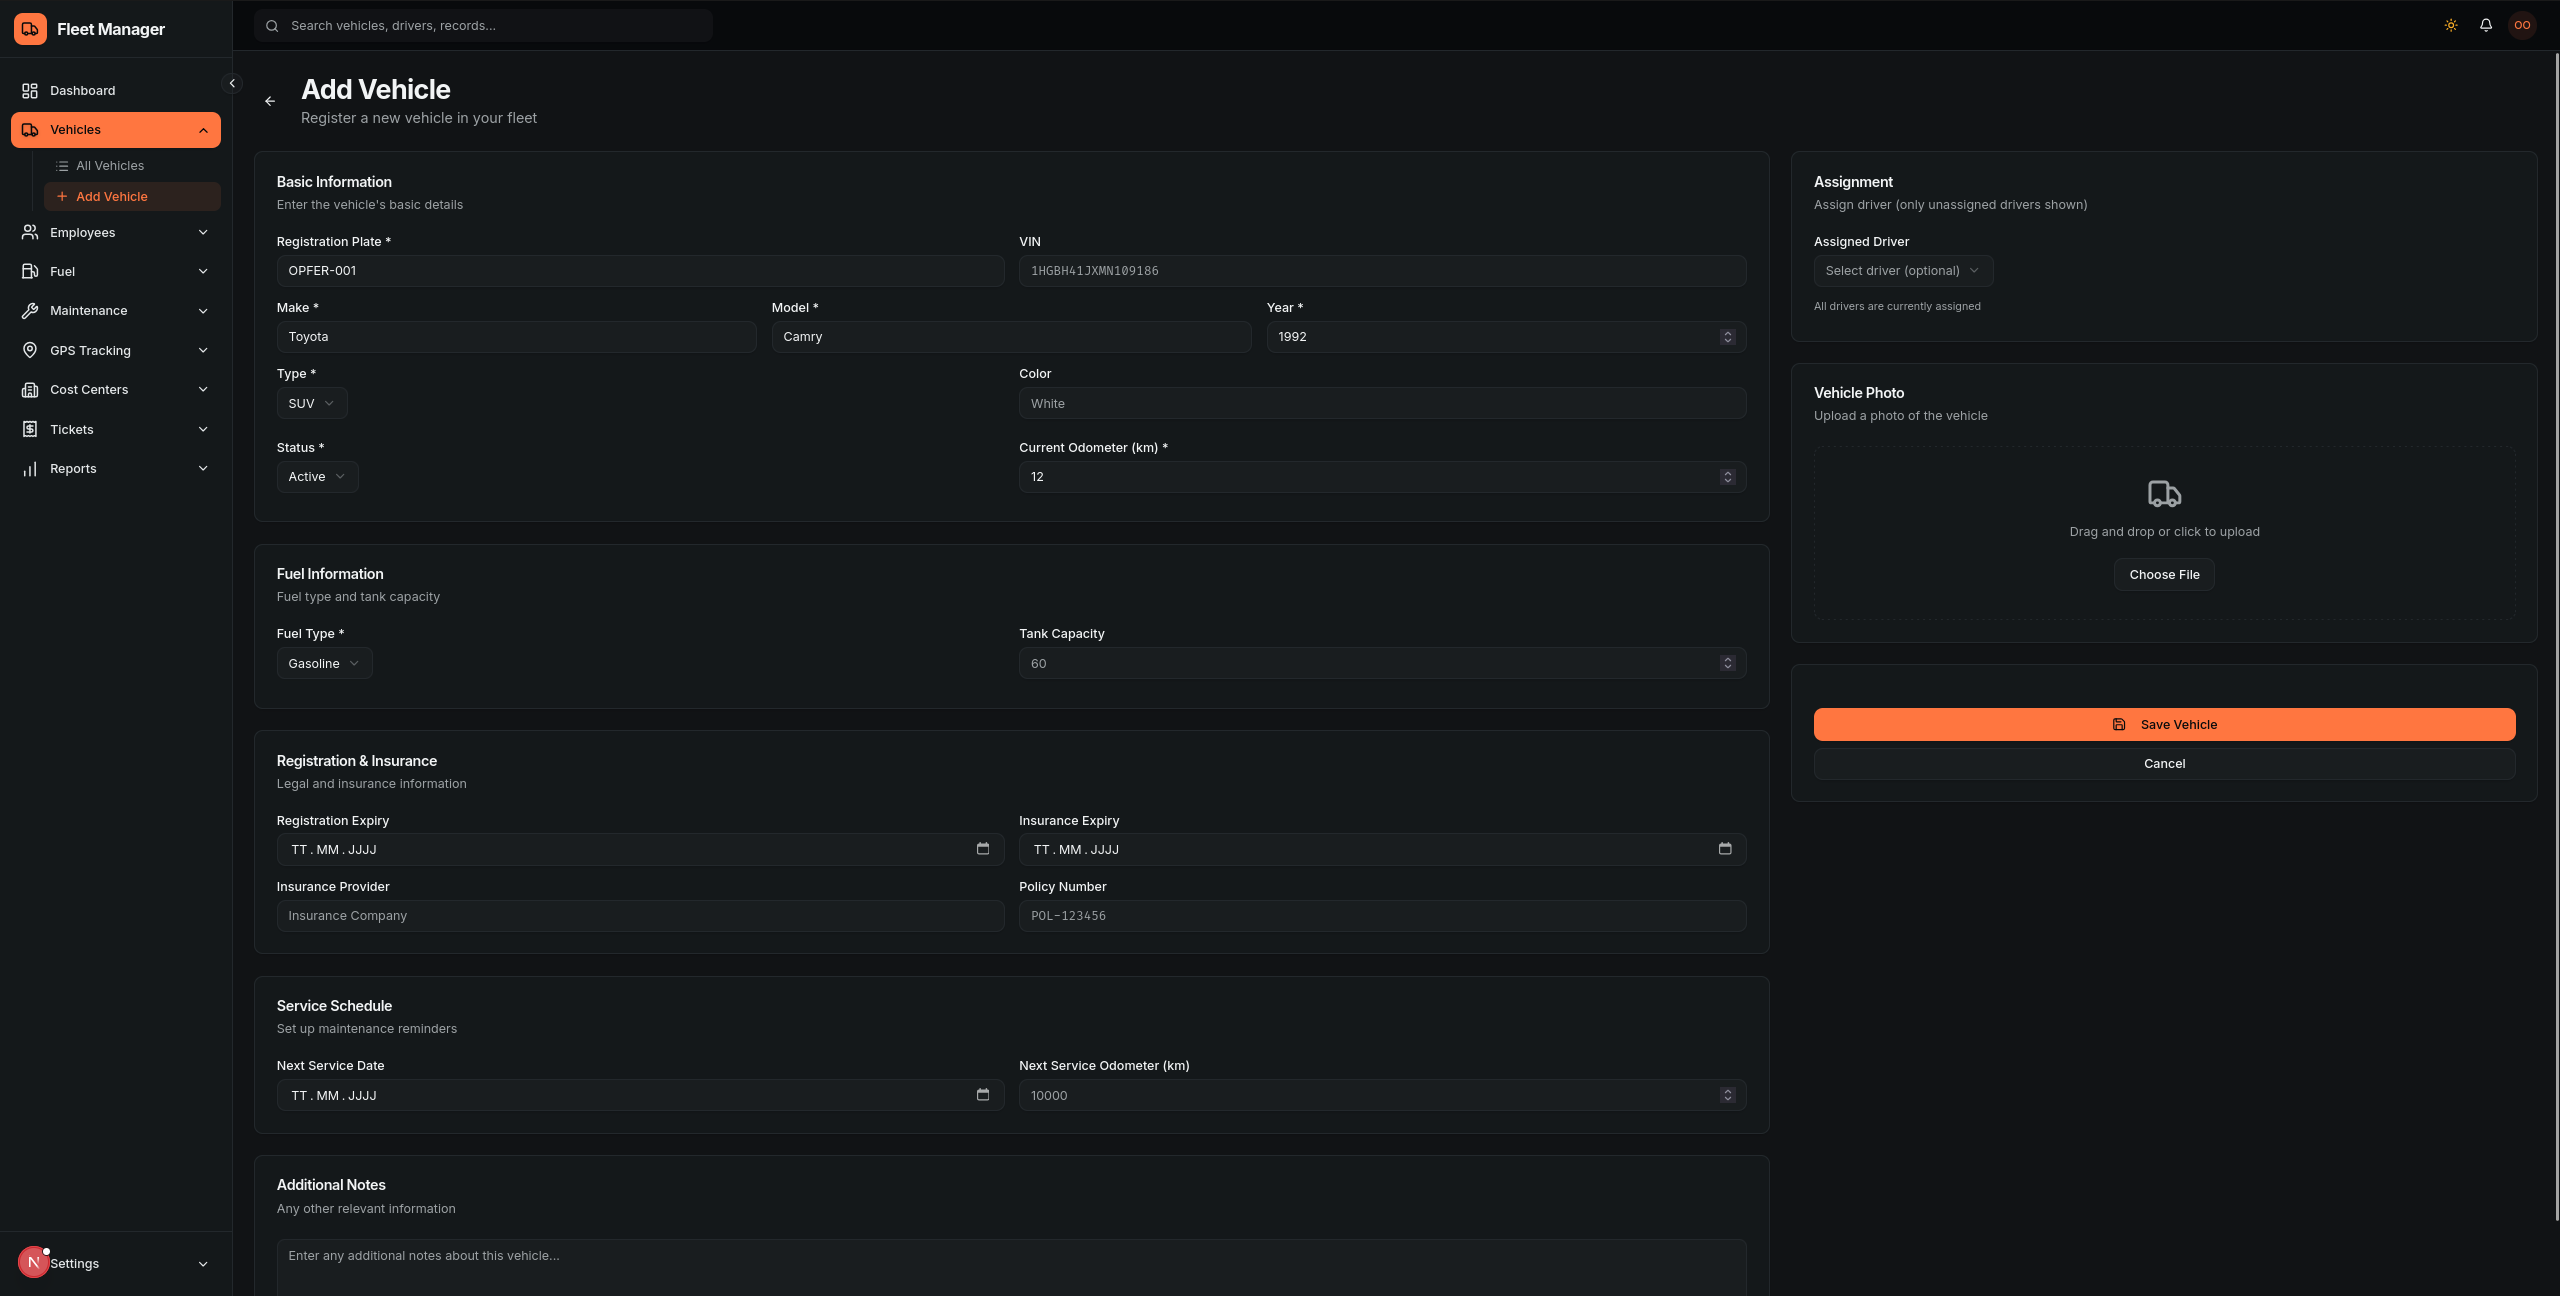
\includegraphics[width=0.9\linewidth]{graphics/ui_attack/opfer_create_vehicle.png}
        \caption{Das Opfer legt im Fleet-Management ein Fahrzeug an.}
        \label{fig:ui-opfer-create-vehicle}
    \end{figure}

    \begin{figure}[H]
        \centering
        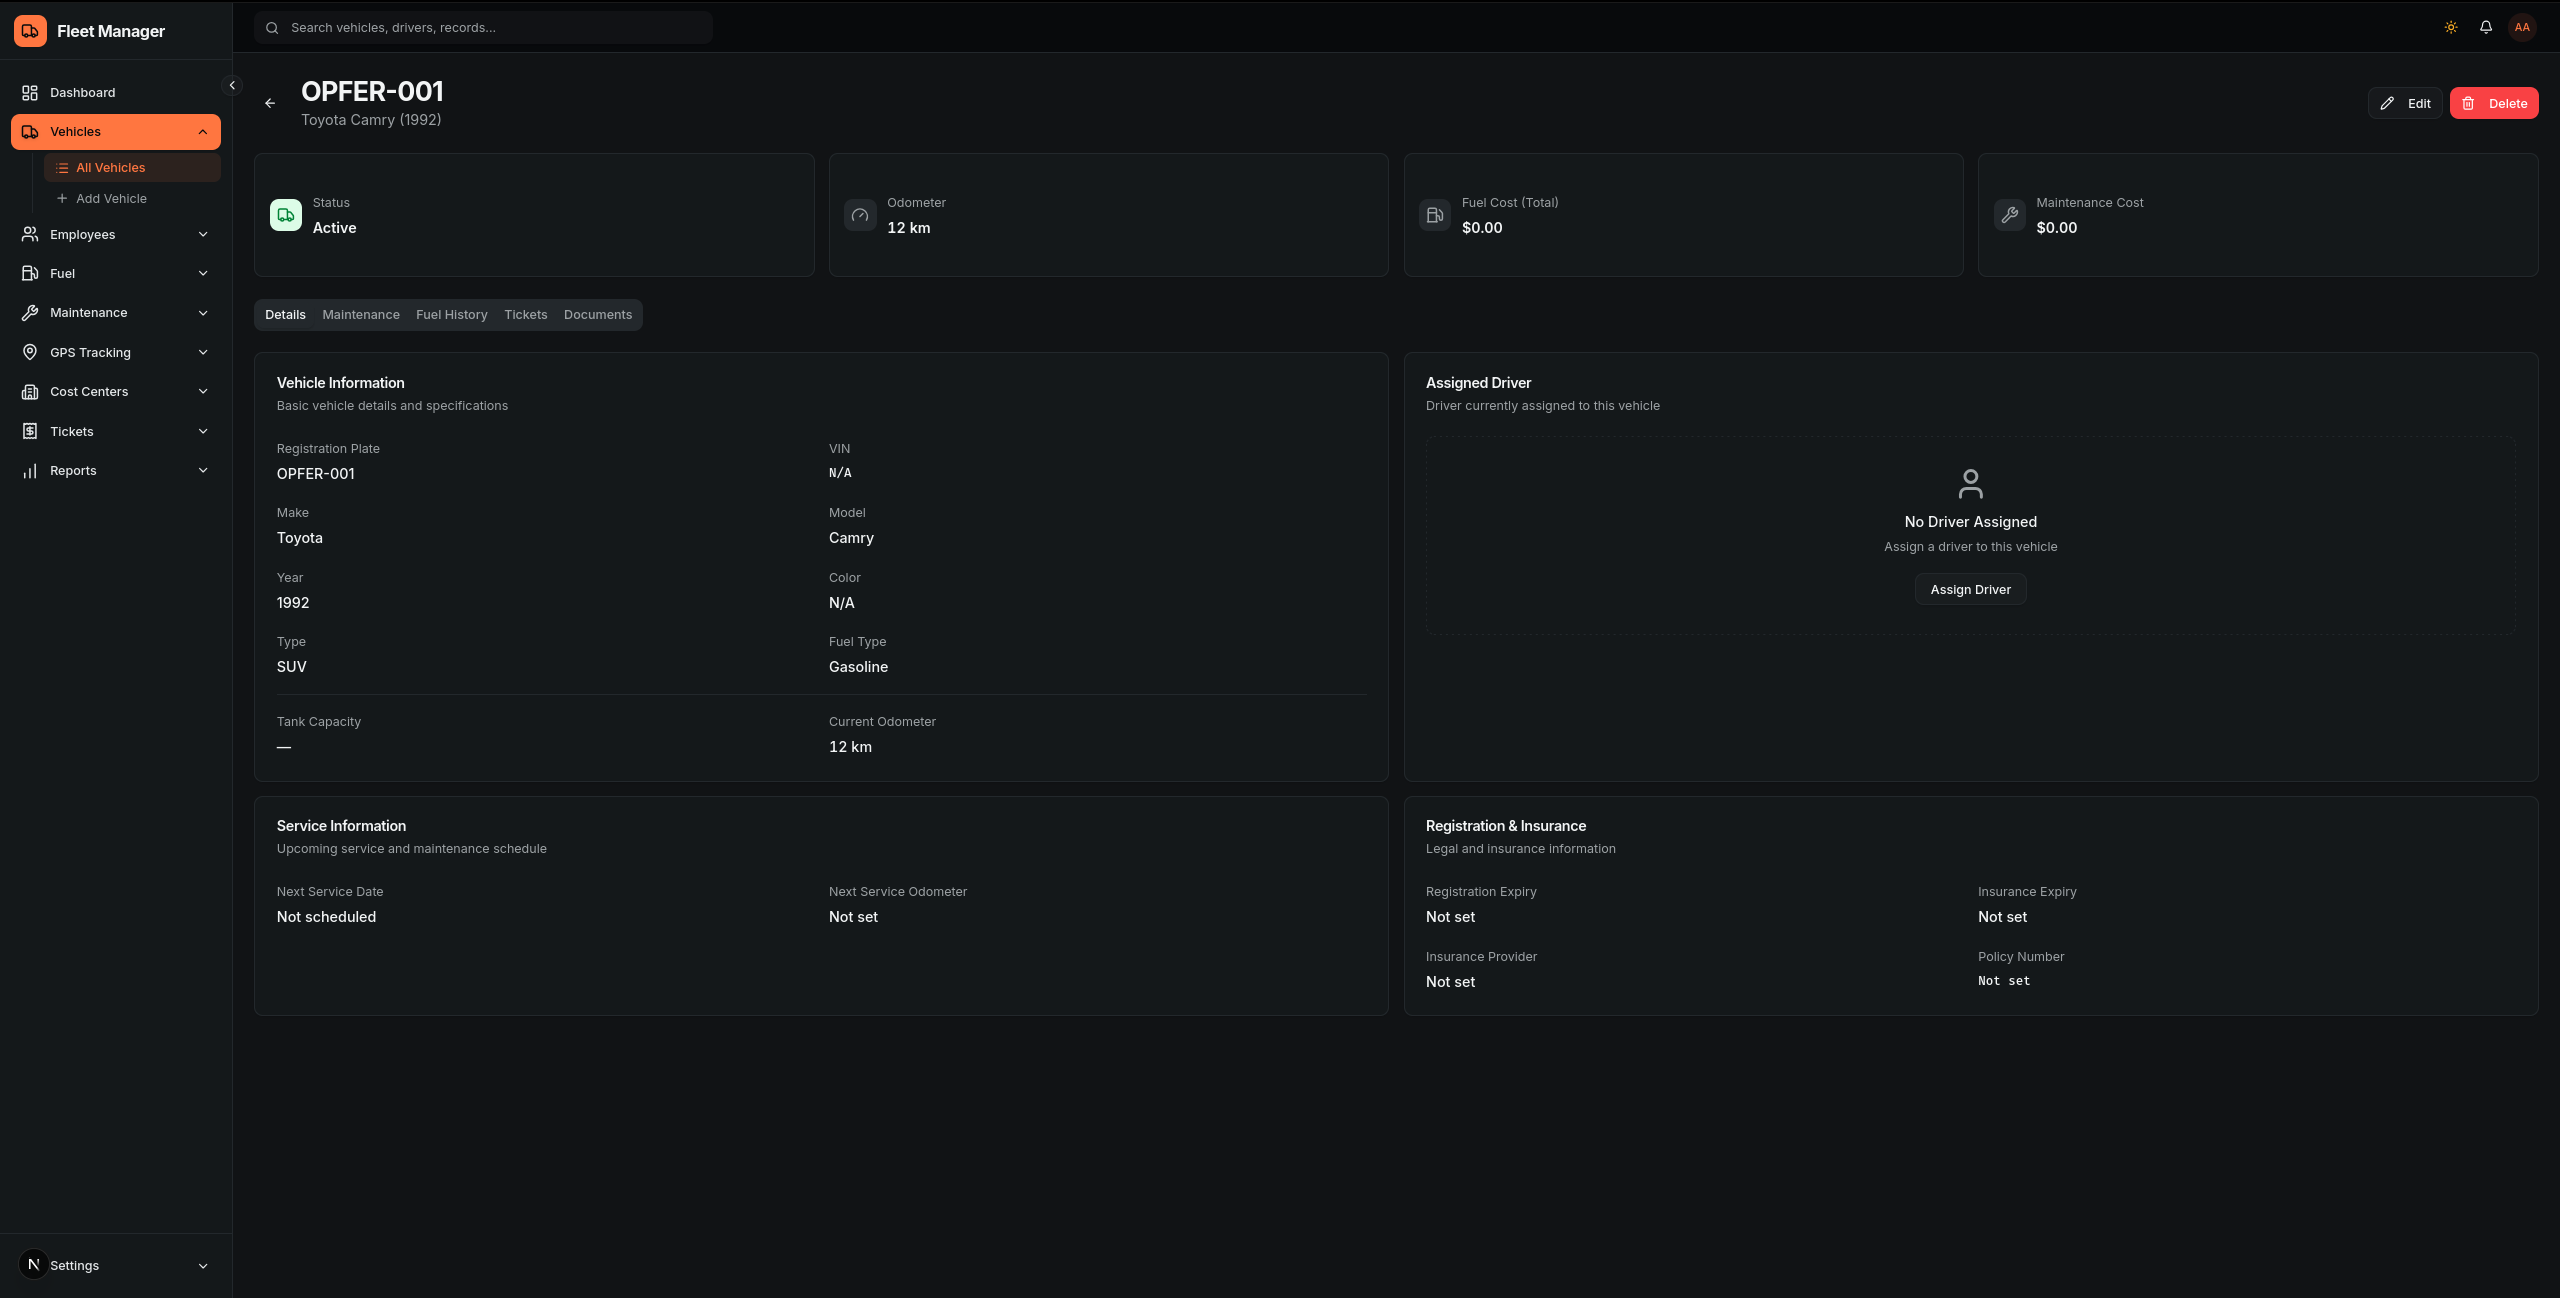
\includegraphics[width=0.9\linewidth]{graphics/ui_attack/angreifer_opfer_vehicle.png}
        \caption{Der Angreifer kann das Fahrzeug des Opfers über die direkte Objekt-ID aufrufen.}
        \label{fig:ui-angreifer-opfer-vehicle}
    \end{figure}

    \begin{figure}[H]
        \centering
        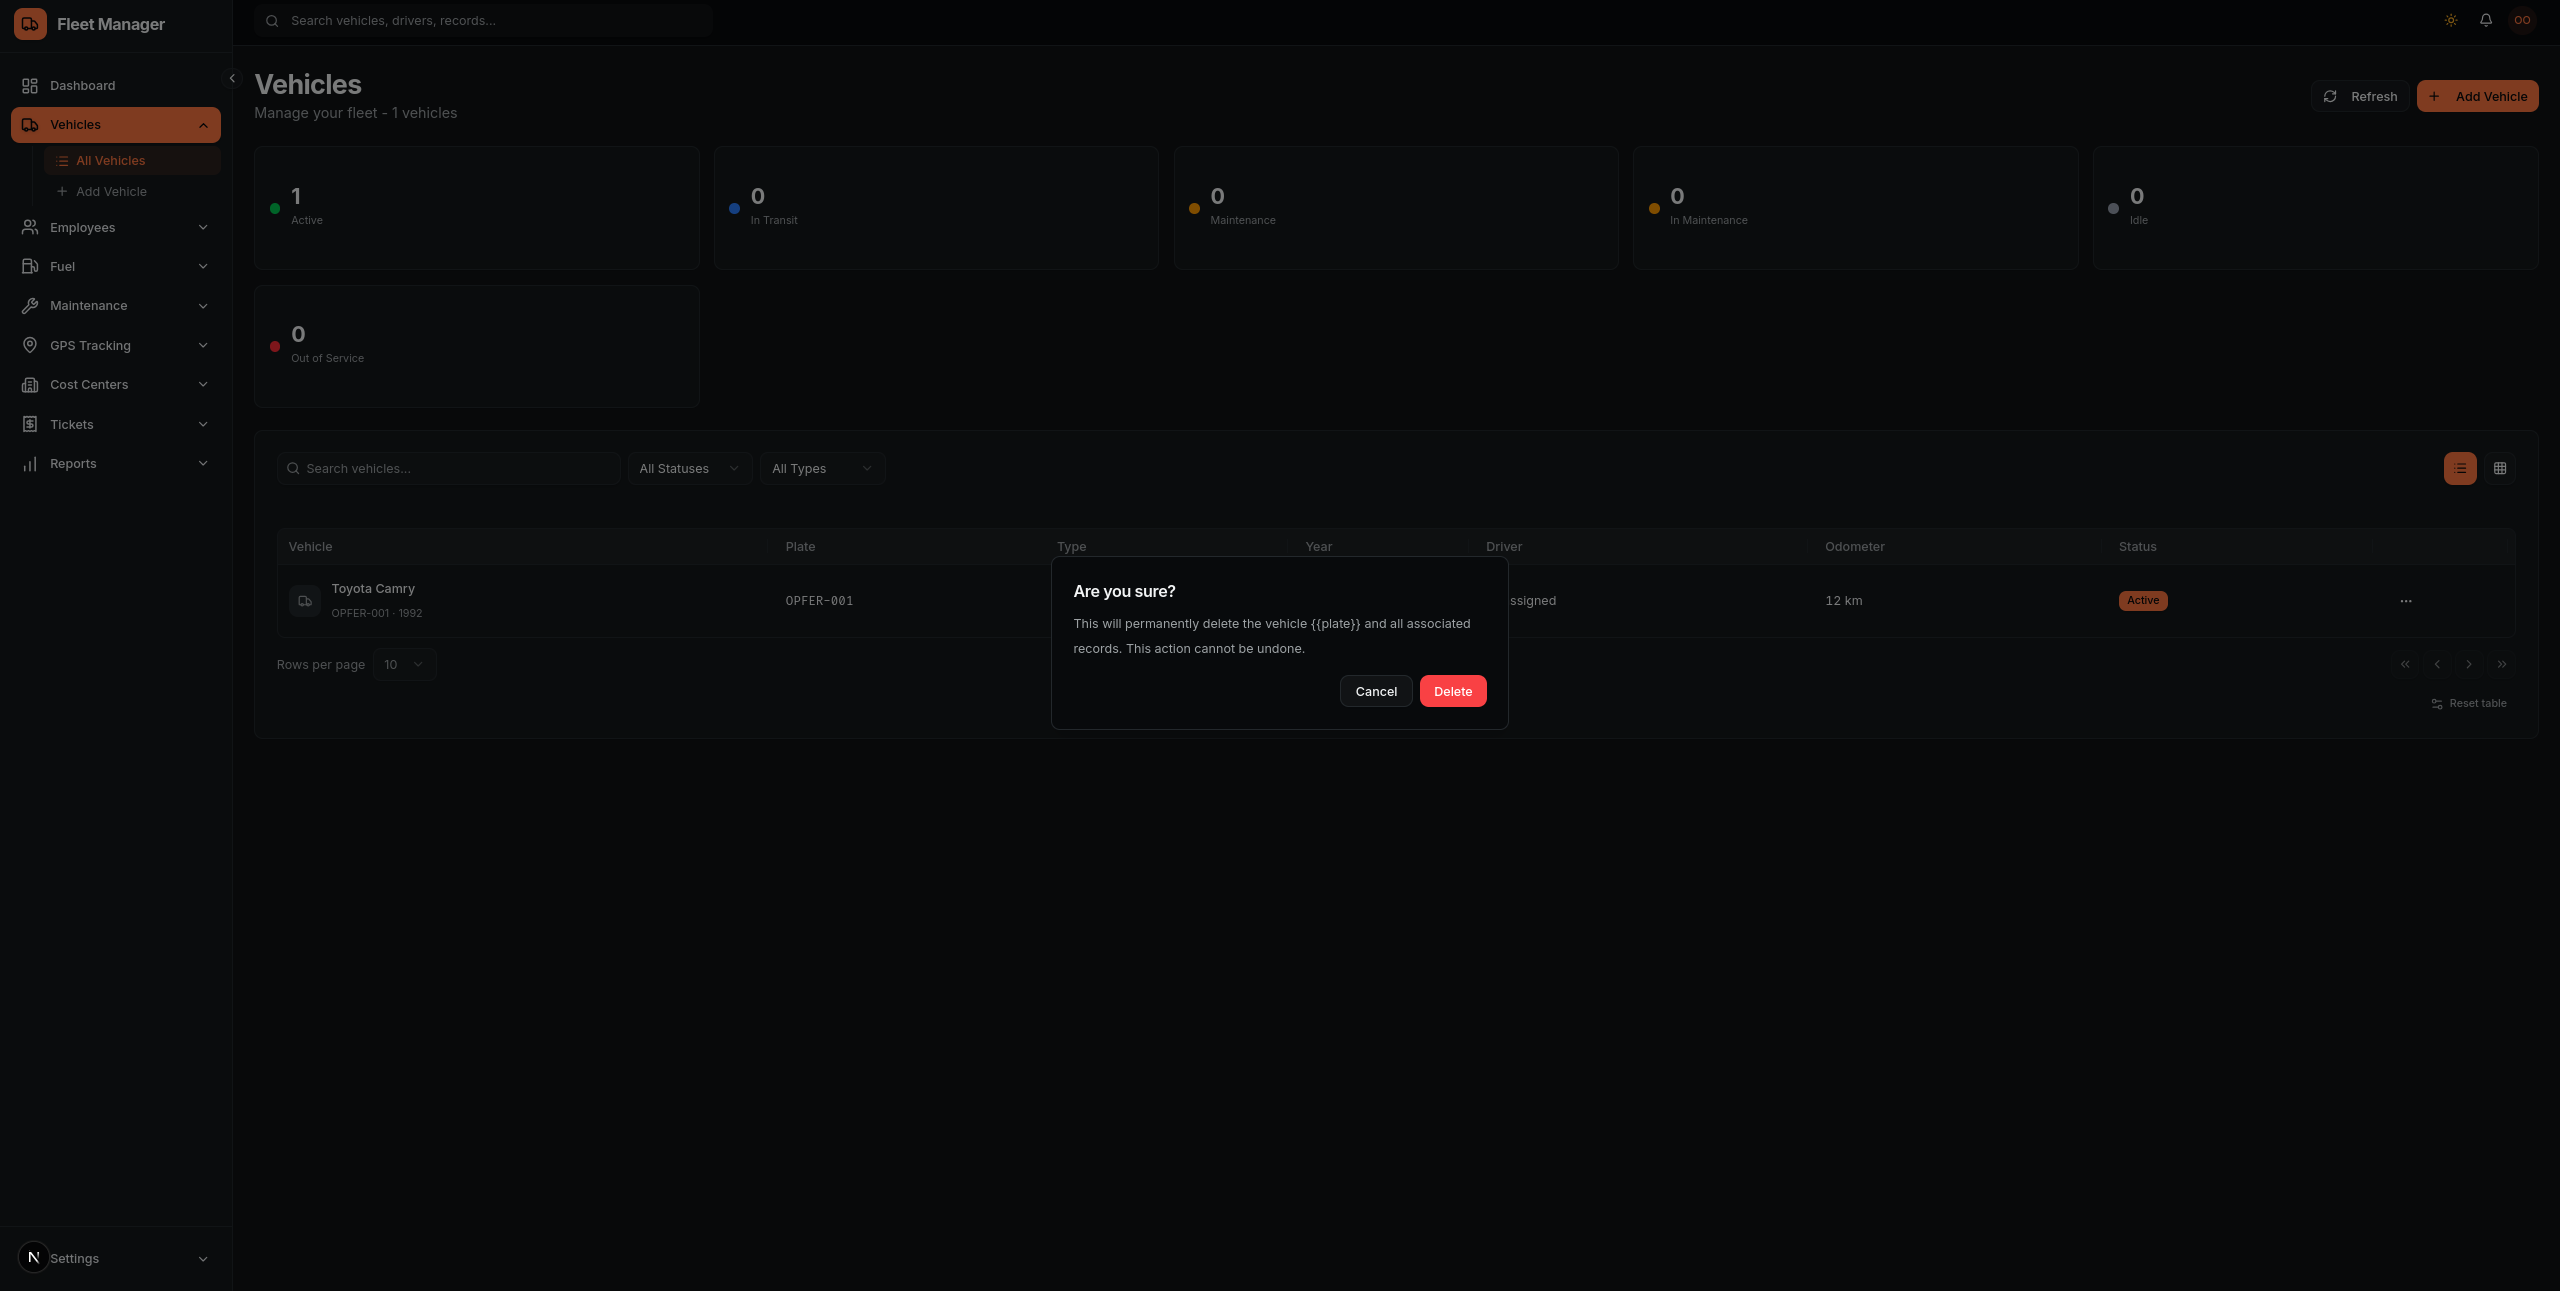
\includegraphics[width=0.9\linewidth]{graphics/ui_attack/opfer_softdelete.png}
        \caption{Soft-gelöschte Datensätze bleiben vor dem Patch in der Oberfläche weiterhin erreichbar.}
        \label{fig:ui-softdelete}
    \end{figure}

    \subsection{API-Reproduktion mit curl}

    Die \texttt{curl}-Screenshots zeigen denselben Sachverhalt ohne Frontend. Dadurch
    ist klar erkennbar, dass es sich nicht um ein Anzeigeproblem des Clients,
    sondern um einen serverseitigen Autorisierungsfehler handelt. Das Opfer erzeugt
    ein Fahrzeug, der Angreifer nutzt dessen UUID für einen fremden GET- und
    DELETE-Zugriff, und das Objekt bleibt sogar nach einem Soft-Delete direkt per ID
    lesbar.

    \begin{figure}[H]
        \centering
        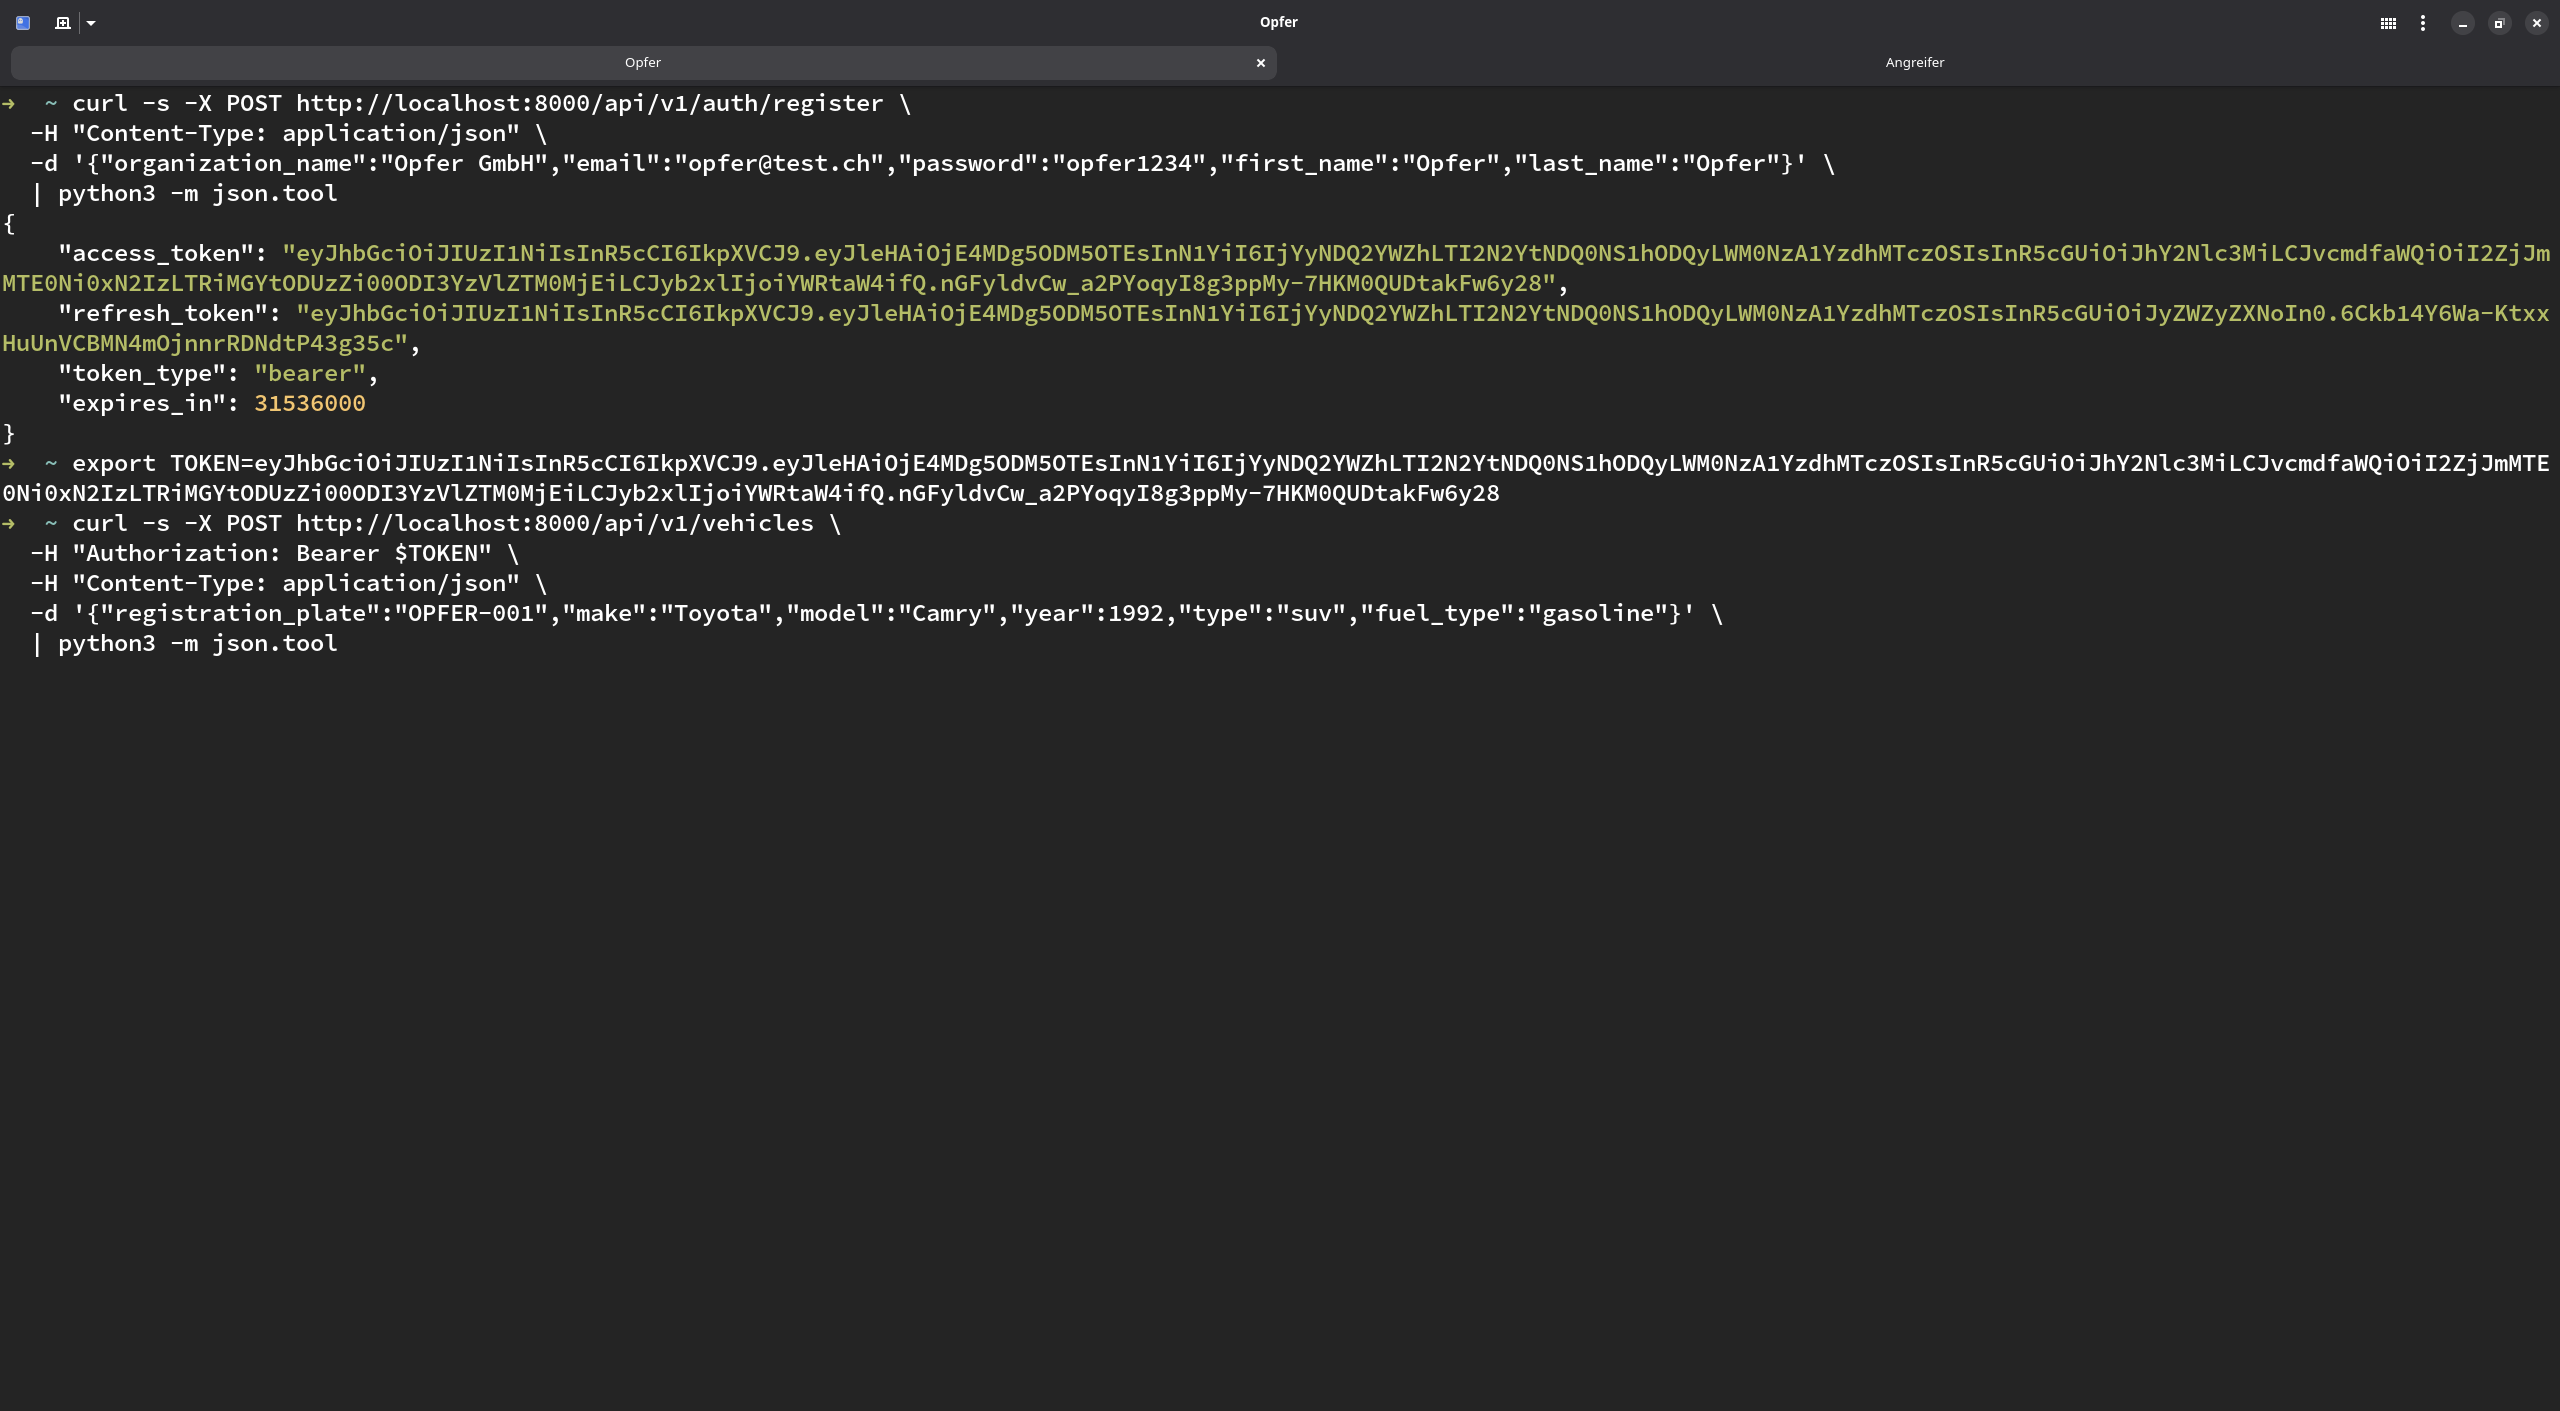
\includegraphics[width=0.9\linewidth]{graphics/curl_attack/opfer_create_vehicle.png}
        \caption{Erzeugung eines Fahrzeugs im Kontext des Opfers per API.}
        \label{fig:curl-opfer-create-vehicle}
    \end{figure}

    \begin{figure}[H]
        \centering
        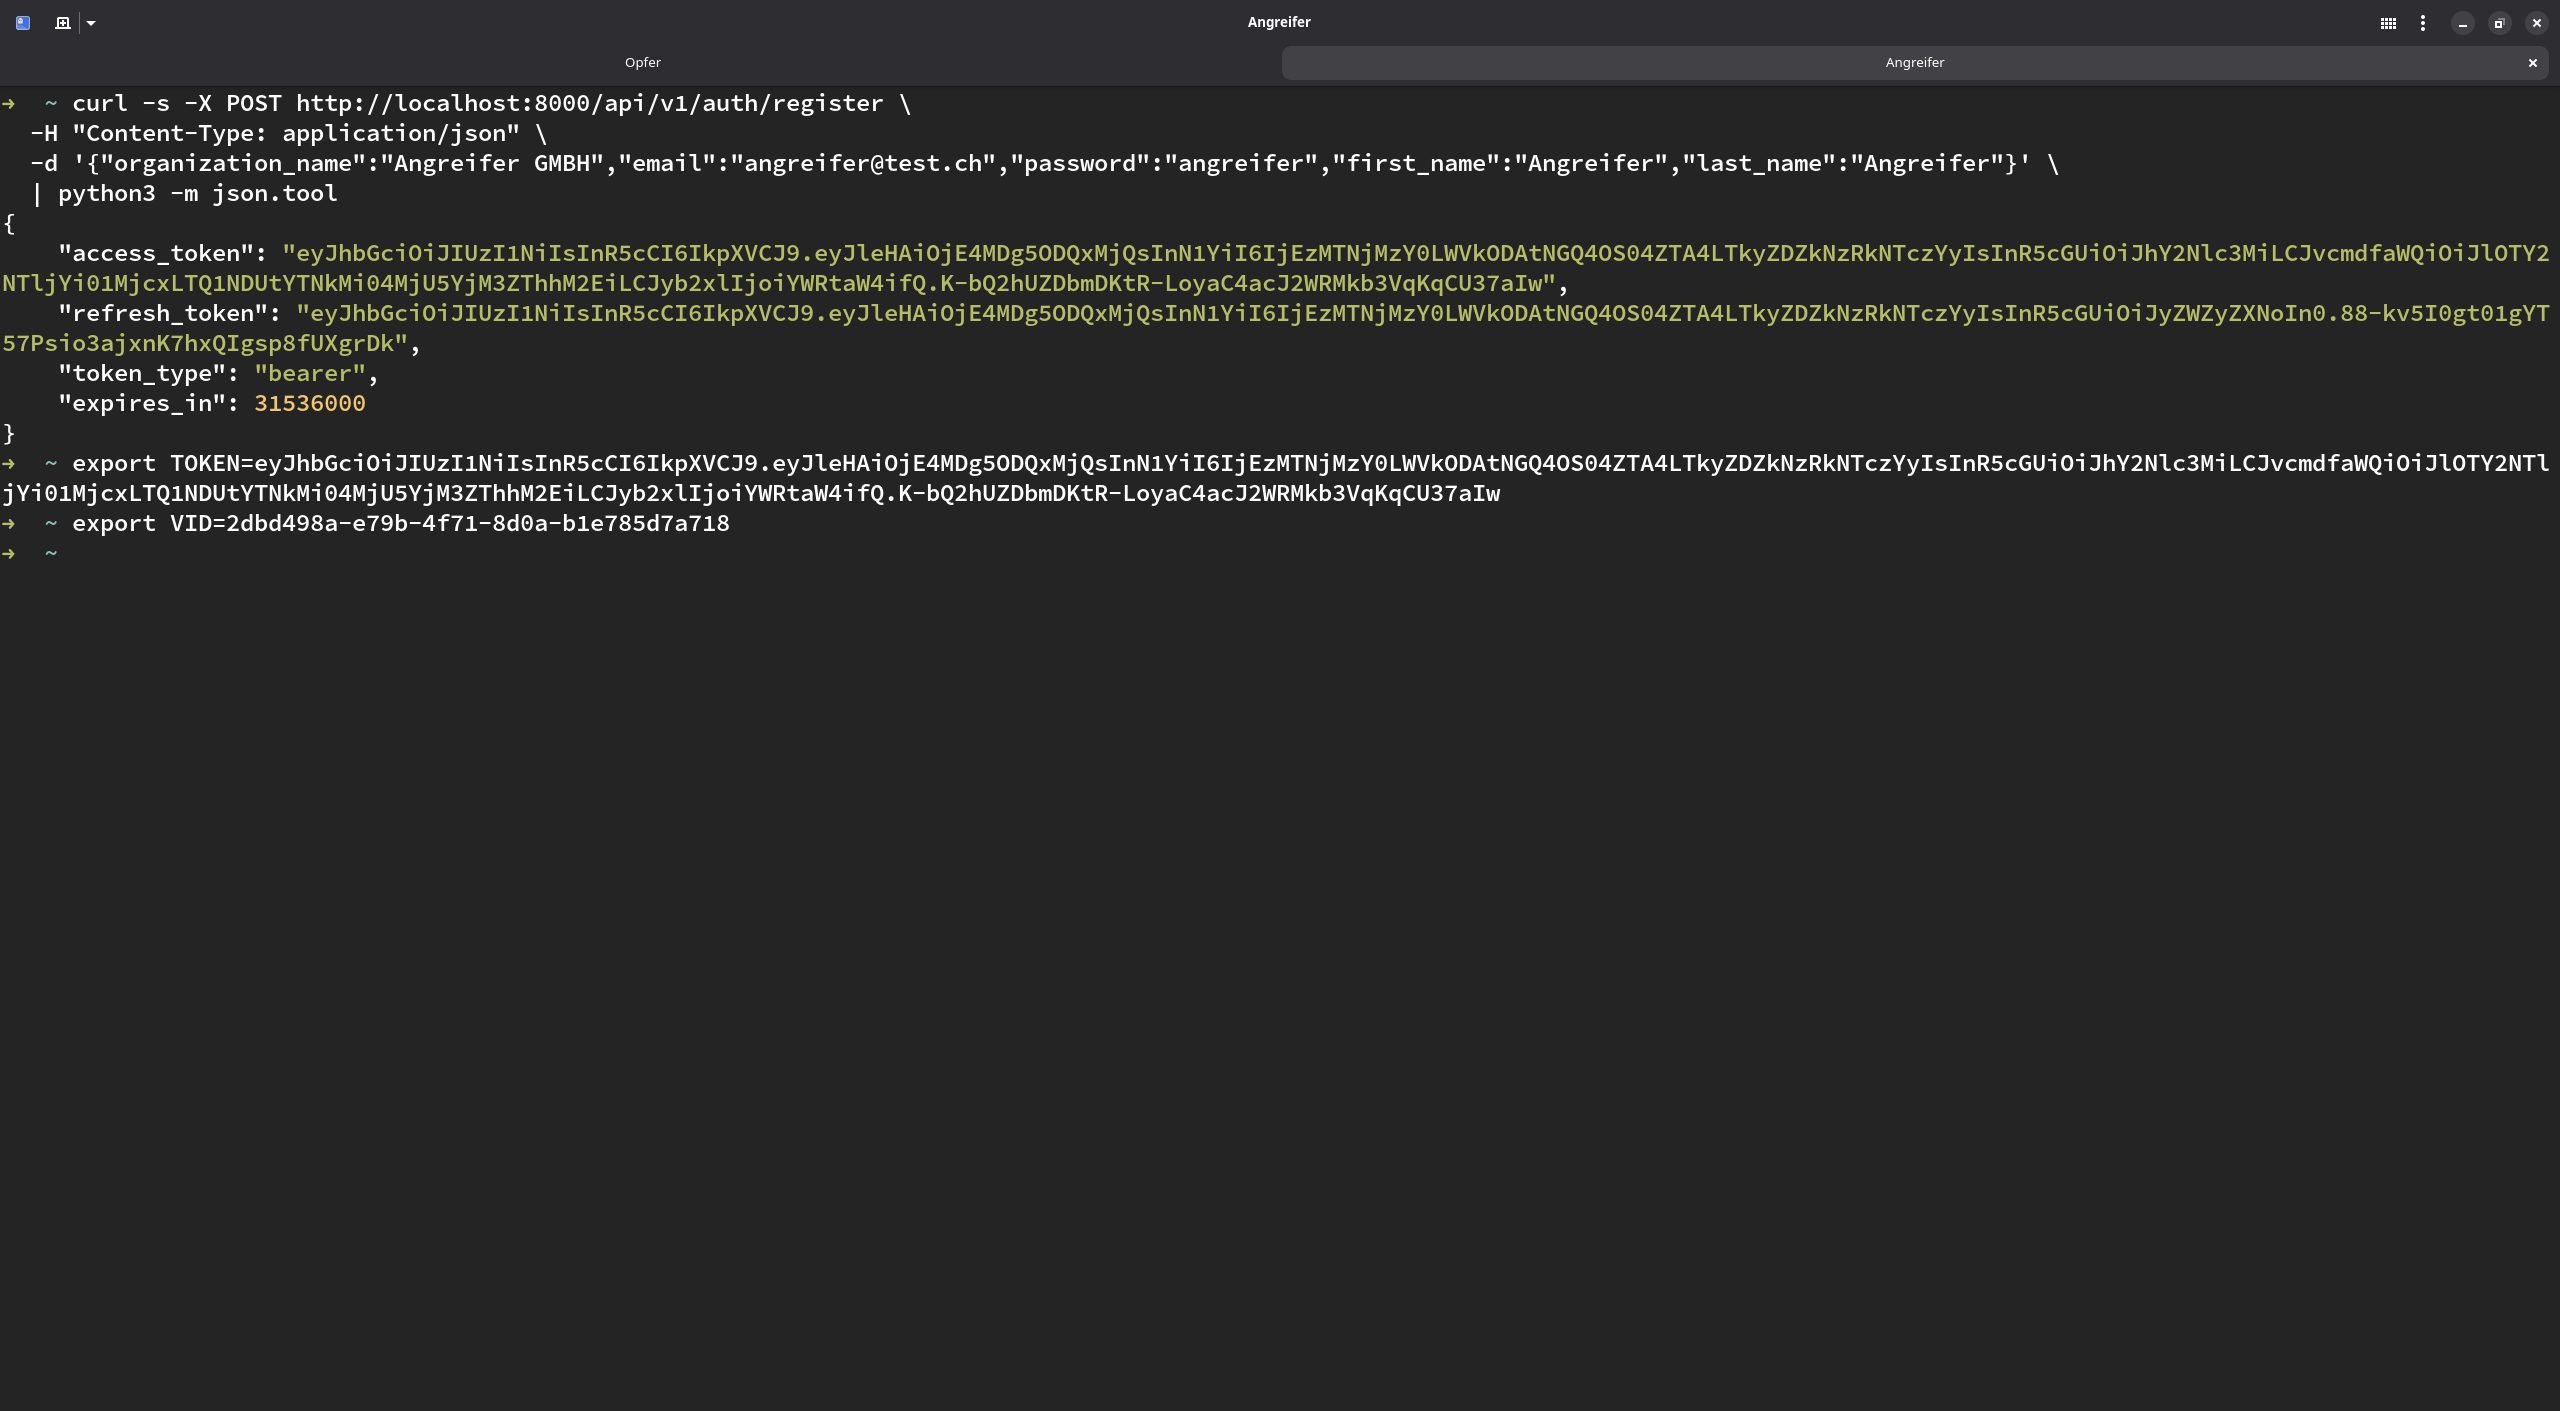
\includegraphics[width=0.9\linewidth]{graphics/curl_attack/use_vehicle_id.png}
        \caption{Der Angreifer verwendet dieselbe UUID für einen unautorisierten GET-Zugriff.}
        \label{fig:curl-use-vehicle-id}
    \end{figure}

    \begin{figure}[H]
        \centering
        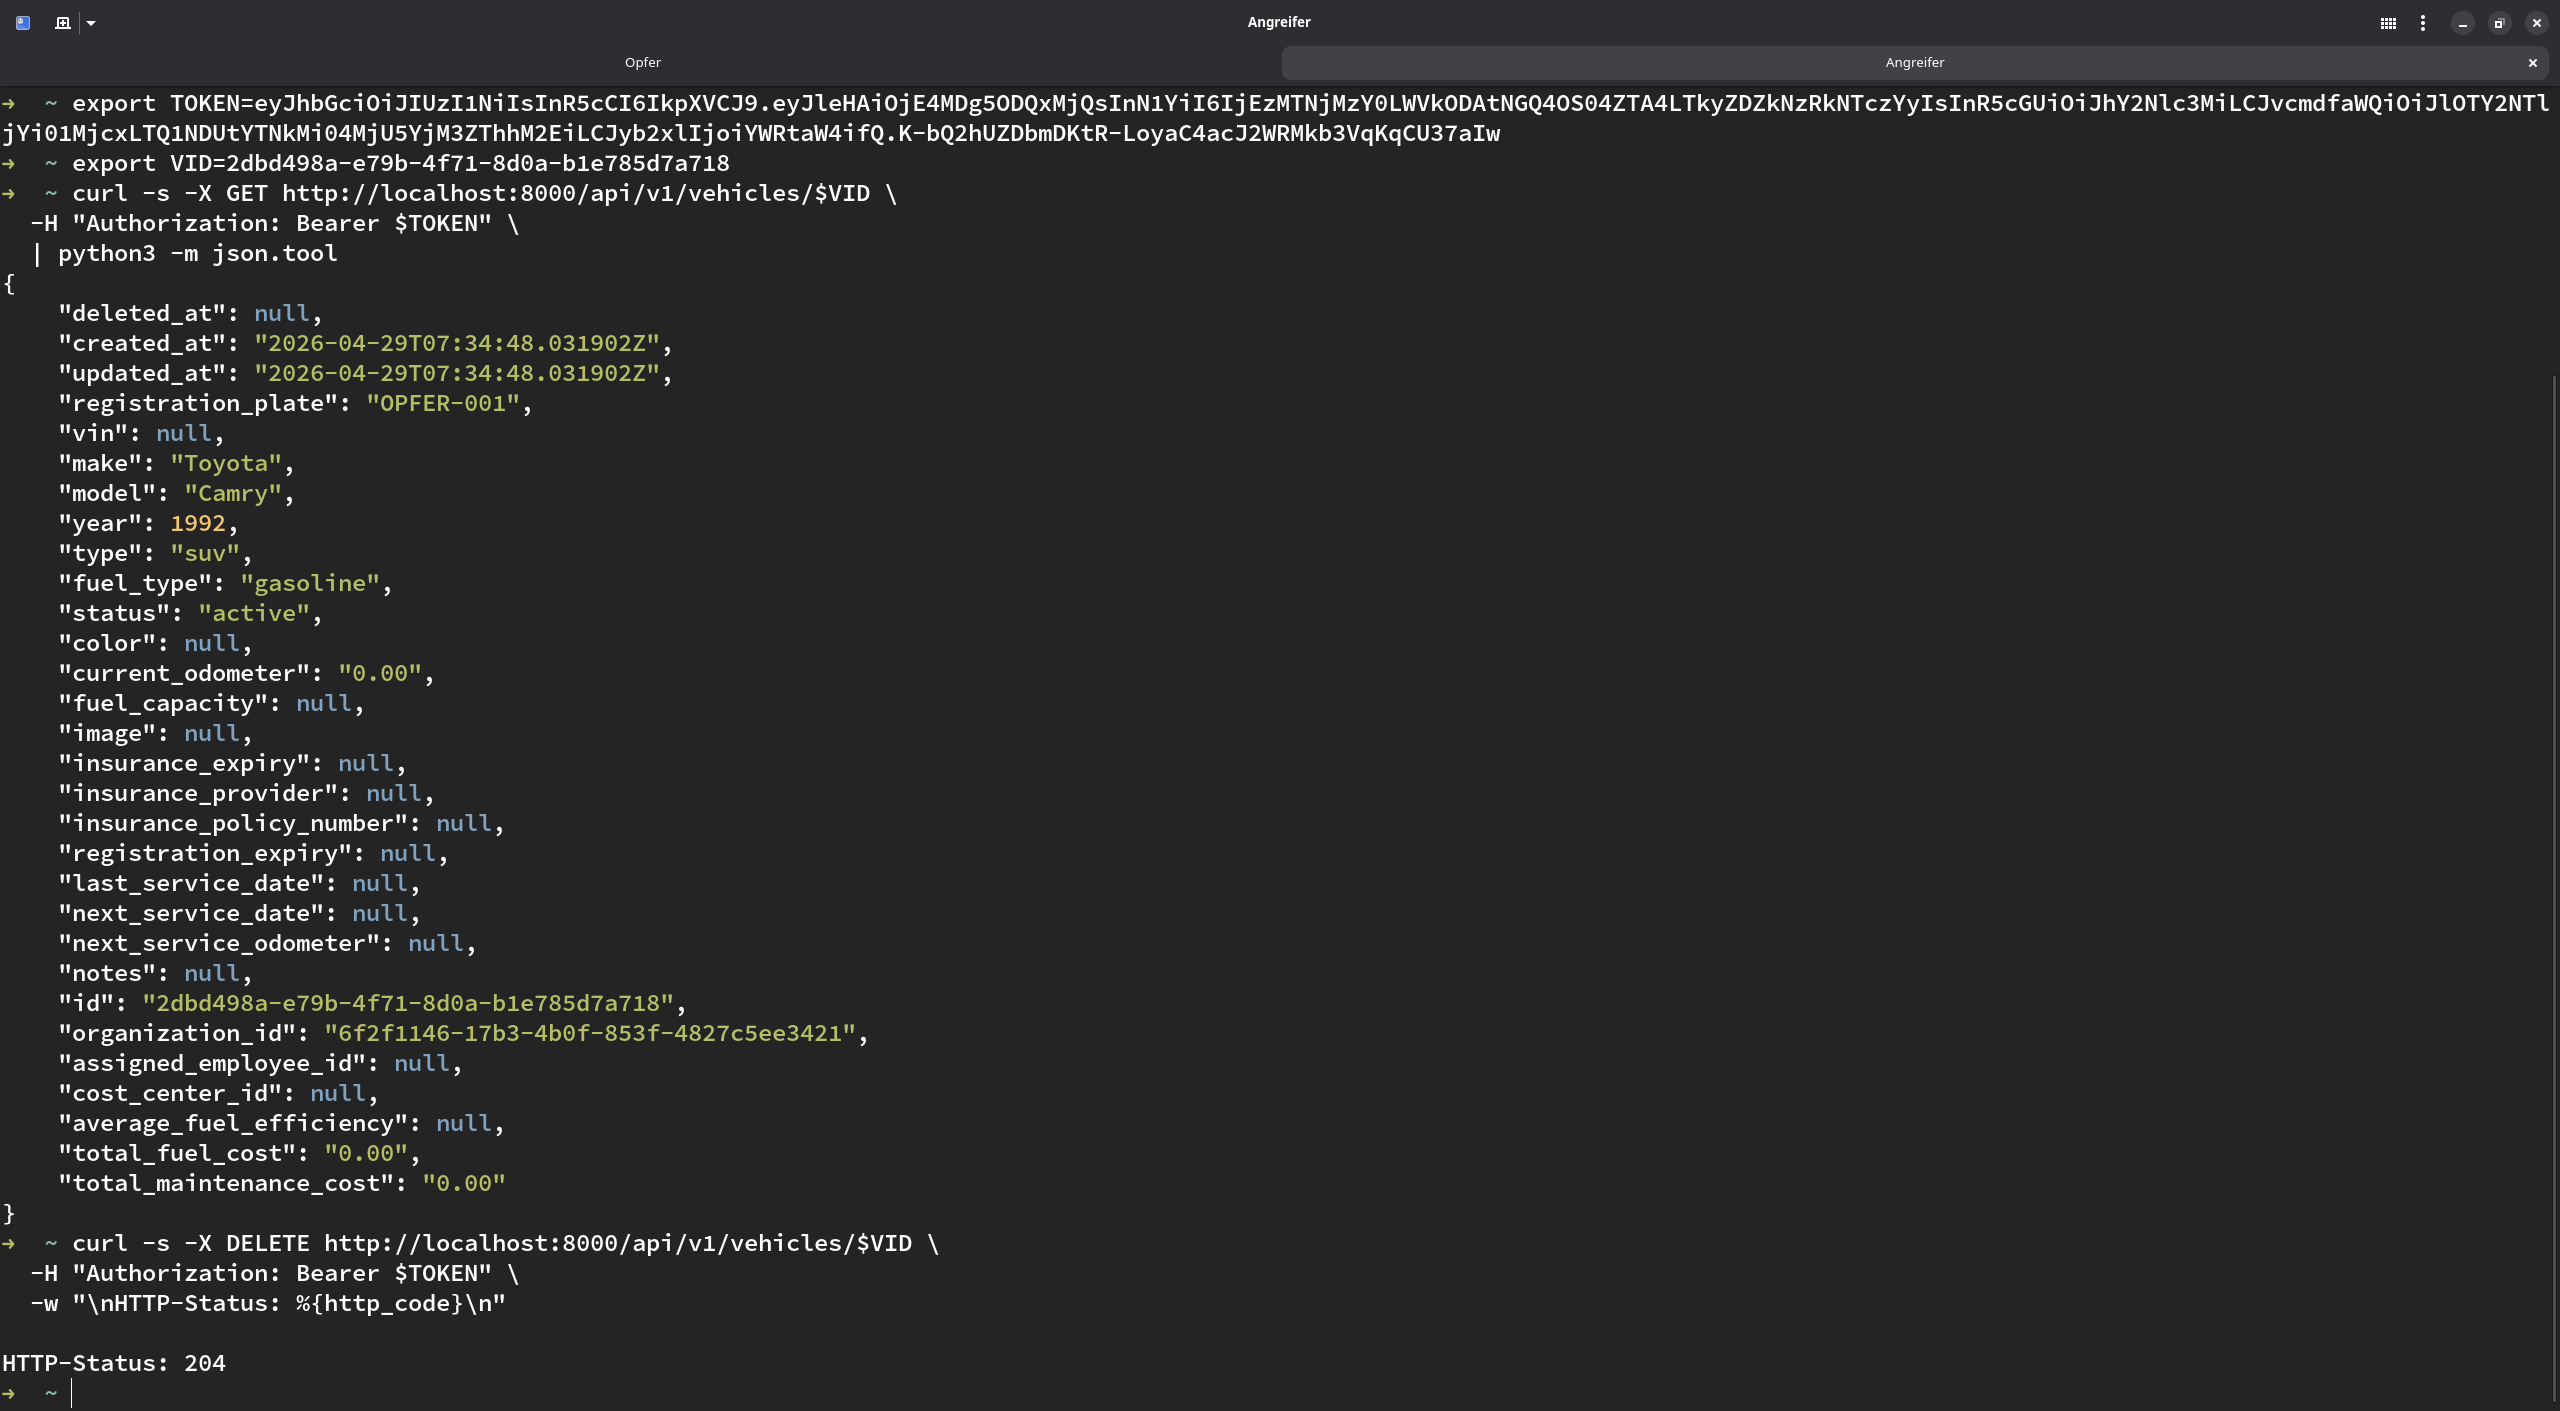
\includegraphics[width=0.9\linewidth]{graphics/curl_attack/angreifer_delete_vehicle.png}
        \caption{Unautorisierter DELETE-Aufruf des Angreifers gegen das Fahrzeug des Opfers.}
        \label{fig:curl-delete-vehicle}
    \end{figure}

    \begin{figure}[H]
        \centering
        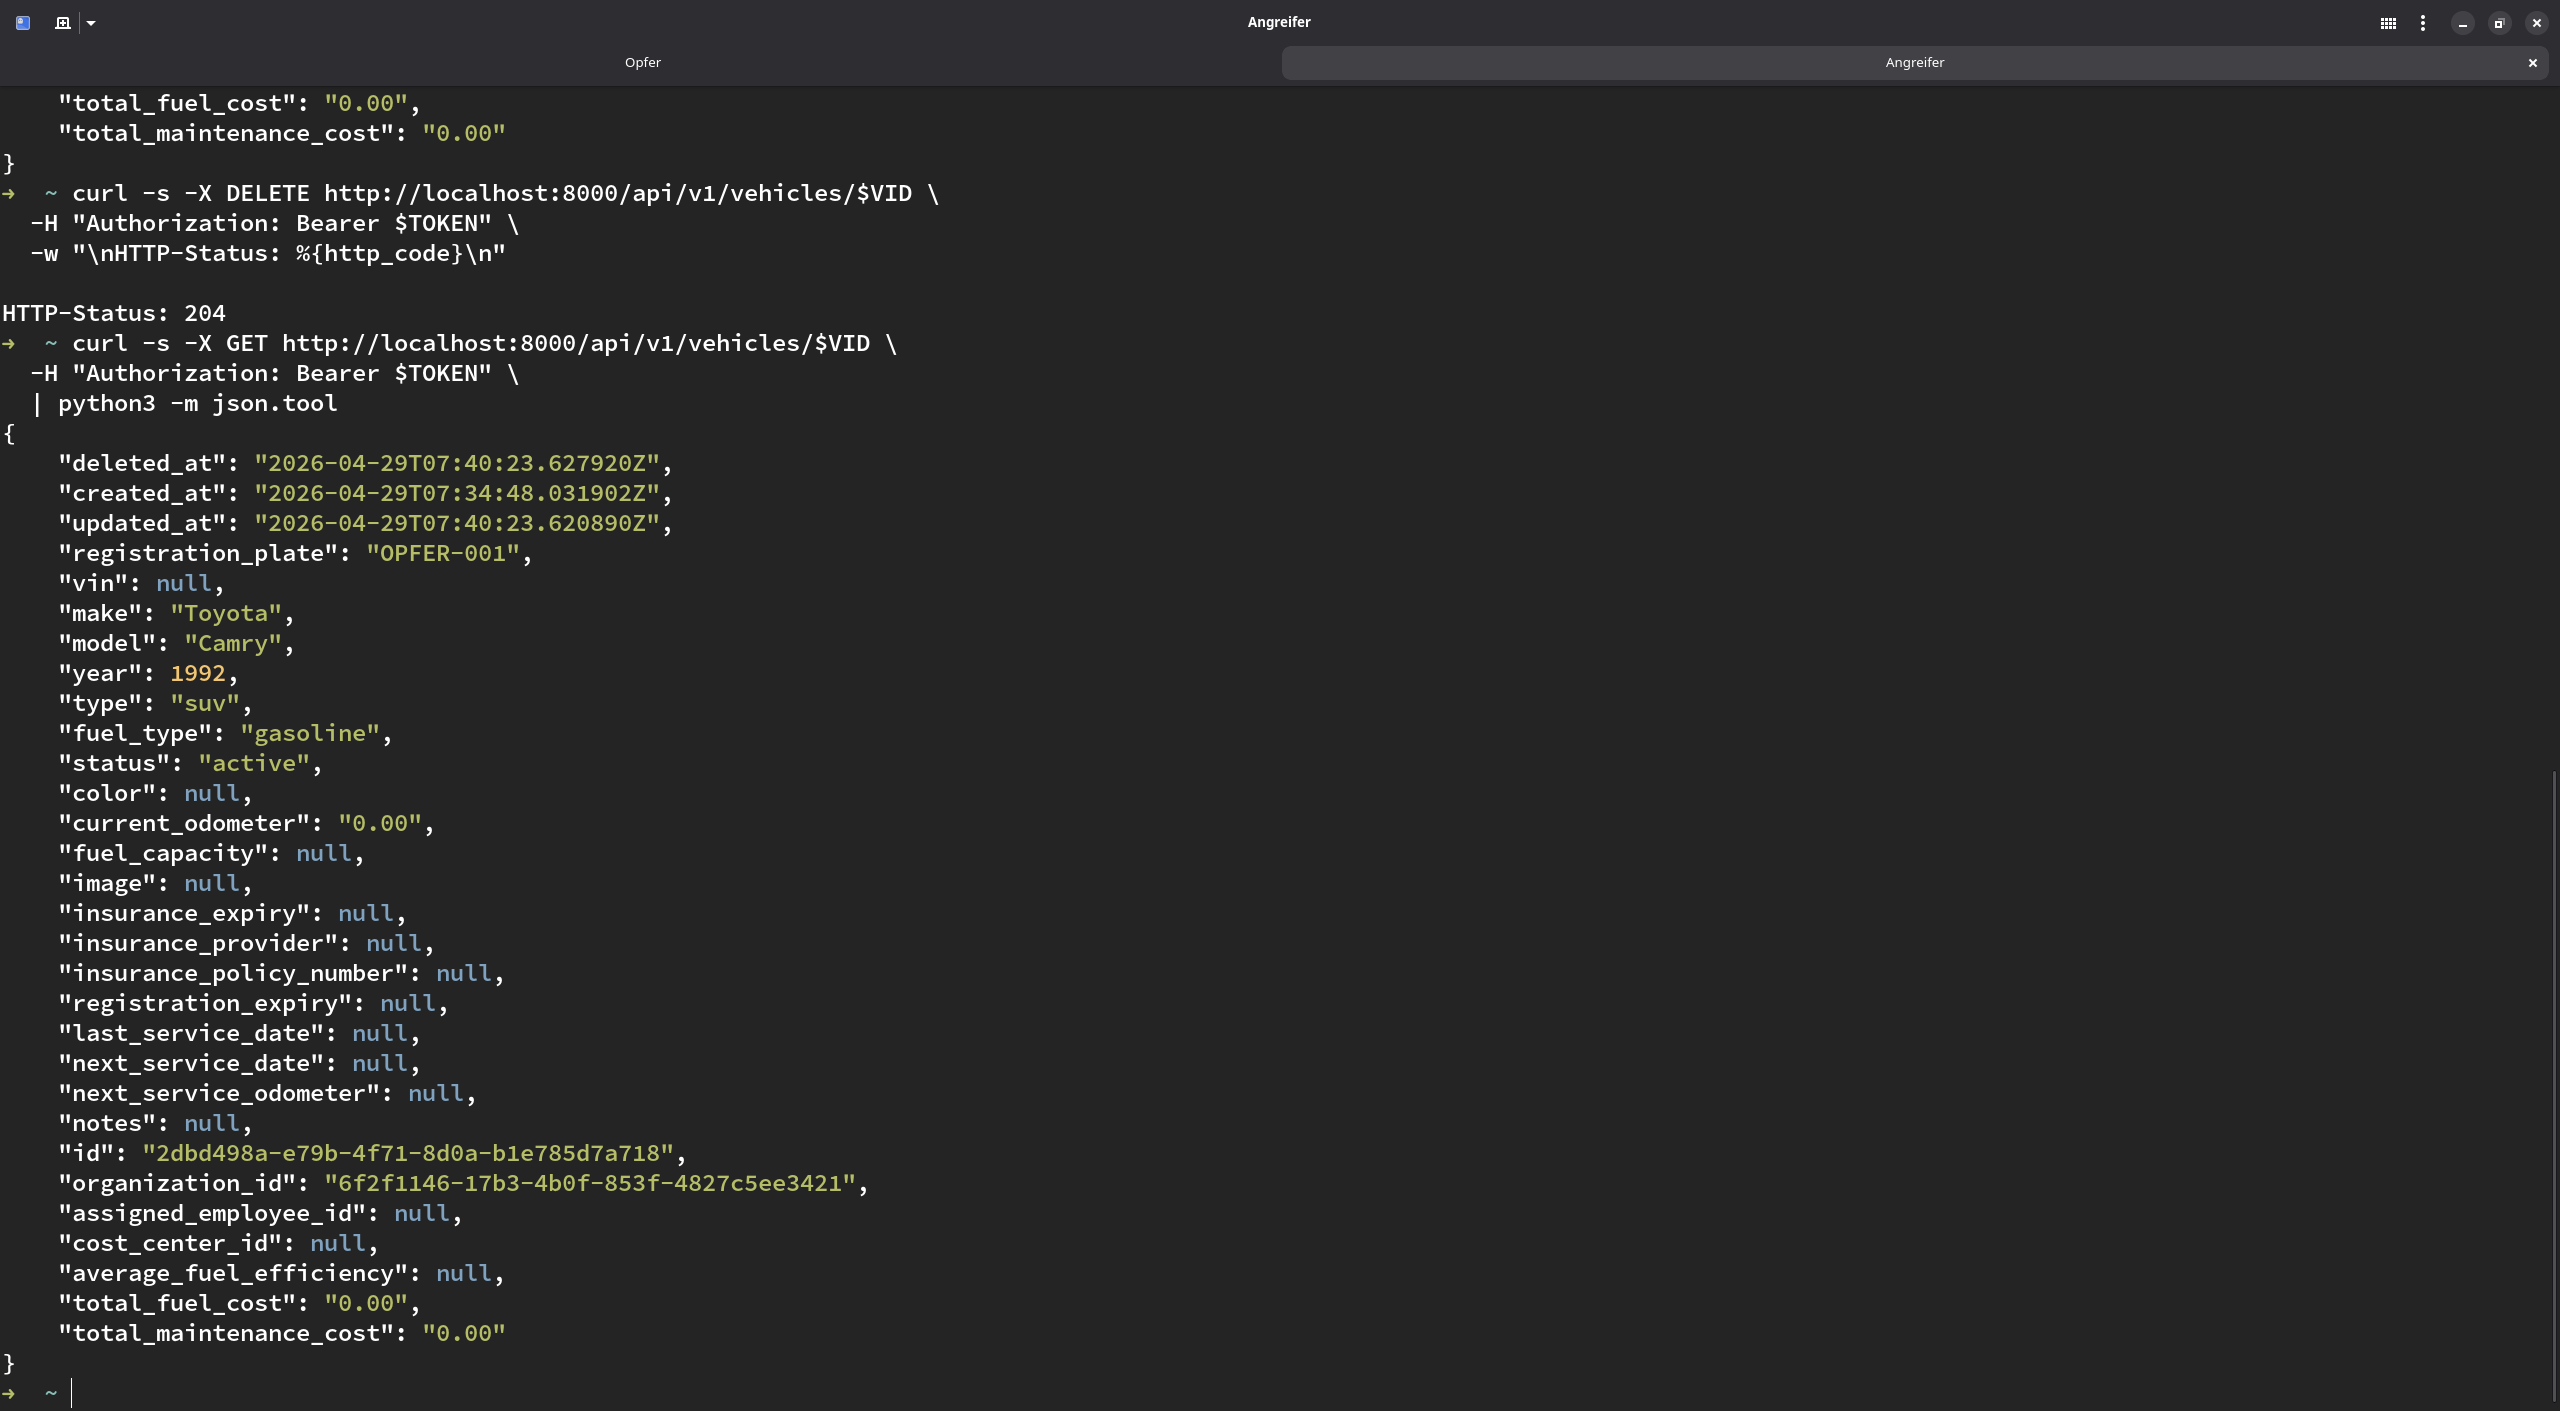
\includegraphics[width=0.9\linewidth]{graphics/curl_attack/vahicle_after_delete.png}
        \caption{Das soft-gelöschte Fahrzeug bleibt vor dem Patch per direkter ID-Abfrage sichtbar.}
        \label{fig:curl-vehicle-after-delete}
    \end{figure}

    %\includepdf[pages={1-2},nup=1x2,landscape=true,scale=0.85,offset=10 -40,pagecommand={\section{Eingefügtes Dokument; zwei Seiten auf einer}\label{app:Aufgabenstellung}\thispagestyle{myheadings}}]{appendix/aufgabenstellung.pdf} \newpage

    %%Bei mehrseitigen Dokumenten die folgenden Seiten ohne Überschrift:
    %\includepdf[pages={3-6},nup=1x2,landscape=true,scale=0.85,offset=10 -40,pagecommand={\thispagestyle{myheadings}}]{appendix/aufgabenstellung.pdf} \newpage

    %\includepdf[pages={1},nup=1x1,landscape=true,scale=0.85,offset=10 -40,pagecommand={\section{Eingefügte PDF-Tabelle}\label{app:Timetable}\thispagestyle{myheadings}}]{appendix/timeline_example.pdf} \newpage

    %%Bei mehrseitigen Dokumenten die folgenden Seiten ohne Überschrift:
    %\includepdf[pages={2-5},nup=1x1,landscape=true,scale=0.85,offset=0 -20,pagecommand={\thispagestyle{myheadings}}]{appendix/timeline_example.pdf} \newpage

\end{appendix}
